\chapter{Preliminary Graph Theory}\label{ch:prelim}

First, let's define some basic concepts of graph theory, starting with the graph itself.

\section{Graphs}

A graph is an algebraic structure most commonly used to describe relationships between objects. There are many definitions of a graph. The most abstract definition of a graph is simply a set $V$ and a relation $R$ on $V$ denoting which elements of $V$ are connected. Graphs in general are \textit{directed}, if $R$ is symmetric, the graph is \textit{undirected}. For the purposes of this work we will be using a geometric definition and generally undirected graphs.

\begin{definition}
    An undirected graph is an ordered pair $G = (V, E)$, where $V$ is a set of \textit{vertices} and $E$ is a set of edges, i. e. a set of unordered pairs of vertices $\forall e \in E: ~ e = (u,v); u,v \in V$.
\end{definition}

\begin{definition}
    A \textit{path} in a graph $G$ from $v$ to $w$; $v,w \in V$ is a sequence of vertices $(u_1, u_2, \dots, u_n); ~ \{u_i ~|~ 1 \leq i \leq n\} \subseteq V$ such that $u_1 = v$, $u_n = w$ and $\{(u_i, u_{i+1}) ~|~ 1 \leq i \leq n-1\} \subseteq E$. A graph is \textit{connected} if there exists a path between every pair of vertices $v,w \in V; ~ v \neq w$.
\end{definition}

\begin{definition}
    A \textit{degree} $\Delta (v)$ of a vertex $v$ denotes how many edges are incident to this vertex. $\Delta(G)$ is the highest degree of any vertex in $G$.
\end{definition}

\begin{definition}
    A graph is \textit{k-regular} if the degree of each vertex is exactly $k$. A \textit{cubic graph} is a 3-regular graph.
\end{definition}

As an example, the $K_4$ graph is cubic.

\begin{figure}[h]
    \centering
        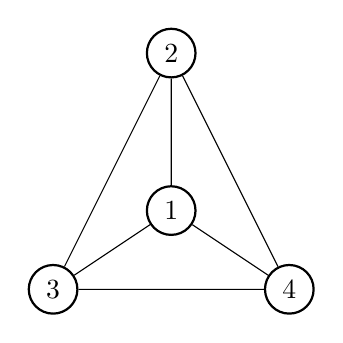
\begin{tikzpicture}
            \begin{scope}[every node/.style={circle,thick,draw}]
                \node (1) at (0,0) {1};
                \node (2) at (0,2) {2};
                \node (3) at (-1.5,-1) {3};
                \node (4) at (1.5,-1) {4};
            \end{scope}
            \draw (1) -- (2) -- (3) -- (4) -- (1) (2) -- (4) (1) -- (3);
        \end{tikzpicture}
\end{figure}

In general statements about graphs in later chapters, we are referring to unordered cubic graphs.

\subsection{Coloring}

When simple binary relationships between objects are not enough, weighted graphs and coloring offer a wider range of applications. Assigning colors to vertices or edges of graphs makes classifications of these objects possible.

\begin{definition}
    A vertex coloring of a graph $G$ is a mapping from the vertex set of $G$ to a set of colors $C$. An edge coloring of a graph $G$ is a mapping from the edge set of $G$ to a set of colors $C$.
\end{definition}

\begin{definition}\label{proper-coloring}
    A \textit{proper vertex coloring} of $G$ is a vertex coloring such that no two neighboring vertices share a color. A \textit{proper edge coloring} is an edge coloring such that no two edges that share an endpoint have the same color. A proper coloring using $k$ colors is called a \textit{k-coloring}.
\end{definition}

As coloring in general is not very interesting, we will be considering only proper colorings henceforth. It is also important to define the set of "colors", especially when coloring signed graphs. Although actual colors tend to be a nice visualization of a coloring, it is more practical to use a subset of integers $C \subseteq \mathbb{Z}$.

The canonical coloring problem is to find the minimum number of colors required for a proper coloring. This number is called the \textit{chromatic number} for vertex colorings and \textit{chromatic index} for edge colorings. Determining the chromatic number and index is useful in other areas of graph theory as well.

\begin{theorem}\label{th:bipartite}
    A graph is bipartite if and only if it has a proper vertex 2-coloring.
\end{theorem}

For regular unsigned graphs these numbers are known.

\begin{theorem}[Brooks\cite{brooks}]
    The chromatic number of a graph $G$ is $\Delta(G)$ for all graphs except complete graphs and cycles of odd length, where the chromatic number is $\Delta(G) + 1$.
\end{theorem}

\begin{theorem}[Vizing]
    The chromatic index of a simple graph $G$ is $\Delta(G)$ or $\Delta(G) + 1$.\todo{cite}
\end{theorem}

In other words, we can always color the edges of a graph using at most $\Delta(G) + 1$ colors where $\Delta(G)$ is the highest degree of any vertex in $G$. The lower bound $\Delta(G)$ is trivial; we need exactly $\Delta(G)$ colors at the highest degree vertex in $G$ to construct a proper coloring. The Vizing theorem\todo{CITE VIZING THEOREM} proves the upper bound using Kempe chains.

\section{Signed graphs}

A signed graph is a graph in which each edge has either a positive or a negative sign. There are multiple definitions of a signed graph but for our purposes a sign function is most practical.

\begin{definition}
    A \textit{signed graph} $\Gamma = (G, \sigma)$ consists of a \textit{underlying graph} $G$ and a \textit{sign function} $\sigma : E(G) \rightarrow \{+,-\}$ that assigns a sign to each edge of $G$.
\end{definition}

\begin{figure}[h]
    \centering
        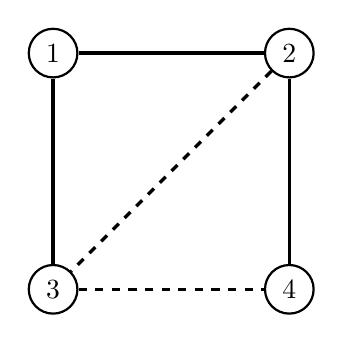
\begin{tikzpicture}
            \begin{scope}[every node/.style={circle,thick,draw}]
                \node (1) at (0,0) {1};
                \node (2) at (3,0) {2};
                \node (3) at (0,-3) {3};
                \node (4) at (3,-3) {4};
            \end{scope}
            \begin{scope}[every edge/.style={draw,very thick}]
                \path
                    (1) edge (2)
                    (2) edge [dashed] (3)
                    (3) edge (1)
                    (2) edge (4)
                    (3) edge [dashed] (4);
            \end{scope}
        \end{tikzpicture}
    \caption[Example of a signed graph]{Example of a signed graph. Dashed lines indicate negative edges, solid lines positive edges.}
\end{figure}

A fundamental concept in the signed graphs theory is \textit{balance}. The sign of a path is the product of the signs of its edges. A path is positive if and only if there is an even number of negative edges on it. A cycle is balanced if it is positive and a signed graph is balanced if each cycle in it is balanced\cite{harary}.

\begin{theorem}[Harary]\label{th:harary}
    A signed graph is balanced if and only if
    \begin{enumerate}
        \item for every pair of vertices, all paths between these vertices have the same sign
        \item the vertices can be divided into two subsets (possibly empty) such that each edge with both ends in the same subset is positive and each edge with ends in different subsets is negative
    \end{enumerate}

    This is a generalization of the earlier mentioned bipartite graph theorem (\Cref{th:bipartite}).
\end{theorem}

The proof uses the method of \textit{switching}. Switching a vertex of a signed graph reverses the sign of each edge incident to it. More generally, switching a signed graph reverses the sign of each edge between a vertex subset and its complement.

We can prove by induction that a signed graph can be switched to an all-positive graph if and only if it is balanced. Both conditions in Harary's theorem apply to all all-positive graphs and graphs that can be switched from an all-positive graph. Consequently, all balanced graphs are equivalent to an all-positive graph, which is an alternative definition of a positive graph. Similarly, we call a graph \textit{antibalanced} if it is equivalent to an all-negative graph, (all cycles of even length in and antibalanced graph are positive and cycles of odd length are negative).

\begin{definition}
    If a signed graph can be obtained from another signed graph by switching, they are considered \textit{equivalent}. For a single underlying graph, switching forms \textit{equivalence classes} of signed graphs. Within a single equivalence class all graphs can be switched to each other.
\end{definition}

It makes sense to study properties of signed graphs that behave consistently under switching. An example of such property is the sign of cycles. Switching a single vertex doesn't change the sign of cycles (cycles containing the vertex reverse signs for two edges resulting in the same product) and switching a set of vertices is equivalent to a sequence of one-vertex-switches (each edge within the set and within the complement gets reversed twice).

\subsection{Coloring}

The research in signed graph coloring was initiated by Zaslavsky\cite{zaslavsky-graphs} in the early 1980s and published in multiple seminal papers\cite{zaslavsky-invariants,zaslavsky-coloring,zaslavsky-colorful}.

\begin{definition}
    A \textit{signed vertex coloring} $\phi(\Gamma)$ of a graph $\Gamma$ is a mapping from the vertex set of $\Gamma$ to a set of signed colors $C$. A \textit{signed edge coloring} $\gamma(\Gamma)$ of a graph $\Gamma$ is a mapping from the set of half-edges (vertex-edge incidences) of $\Gamma$ to a set of colors $C$. Additionally, the half-edges must have the same color on positive edges and opposite colors on negative edges.

    $$(\forall e = (u,v) \in E(\Gamma))~~ \gamma(e, u) = \sigma(e)\gamma(e, v)$$
\end{definition}

\begin{definition}
    A \textit{proper vertex signed coloring} is a coloring $\phi(\Gamma)$ such that for each pair of neighboring vertices $(u,v)$ $\phi(u) \neq \sigma(uv)\phi(v)$. In case of \textit{proper edge signed coloring} the definition remains the same, because the coloring condition is already a part of the general coloring definition. Each color must be present at each vertex at most once (or adjacent half-edges have different colors). We are, again, assuming only proper colorings from now on.
\end{definition}

Here it is even more important to define the color set. Zaslavsky\cite{zaslavsky-coloring} defined a $k$-coloring based on a signed color set $C_k = \{-k, -(k-1), \dots, -1, 0, 1, \dots, (k-1), k\}$ and called colorings zero-free if the color $0$ was not used. He then studied the properties of \textit{chromatic polynomials} related to signed colorings, the number of colorings for a signed graph. (Balanced chromatic polynomials in case of zero-free colorings.)

This definition is consistent under switching. Assuming a graph $\Gamma$ and a proper vertex coloring $\phi$, if we obtain $\Gamma'$ by switching vertex $u$, then $\phi' = \phi; \phi'(u) = -\phi(u)$ is a proper vertex coloring of $\Gamma'$. Similarly for edge coloring in which we reverse the sign of each half-edge incident to $u$.

\begin{figure}[h]
    \centering
    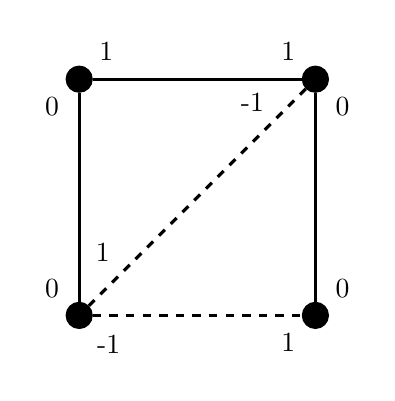
\begin{tikzpicture}
        \begin{scope}[every node/.style={circle,draw,fill=black}]
            \node (1) [label=above right:1, label=below left:0] at (0,0) {};
            \node (2) [label=above left:1, label=below right:0] at (3,0) {};
            \node (3) [label=above left:0, label=below right:-1] at (0,-3) {};
            \node (4) [label=above right:0, label=below left:1] at (3,-3) {};
        \end{scope}
        \node (ar) at (2.2,-0.3) {-1};
        \node (bl) at (0.3, -2.2) {1};
        \begin{scope}[every edge/.style={draw,very thick}]
            \path
                (1) edge (2)
                (2) edge [dashed] (3)
                (3) edge (1)
                (2) edge (4)
                (3) edge [dashed] (4);
        \end{scope}
    \end{tikzpicture}
    \hspace{0.1\textwidth}
    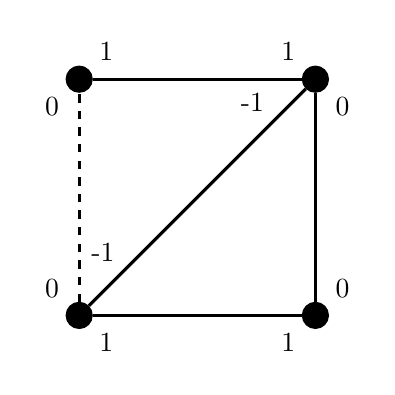
\begin{tikzpicture}
        \begin{scope}[every node/.style={circle,draw,fill=black}]
            \node (1) [label=above right:1, label=below left:0] at (0,0) {};
            \node (2) [label=above left:1, label=below right:0] at (3,0) {};
            \node (3) [label=above left:0, label=below right:1] at (0,-3) {};
            \node (4) [label=above right:0, label=below left:1] at (3,-3) {};
        \end{scope}
        \node (ar) at (2.2,-0.3) {-1};
        \node (bl) at (0.3, -2.2) {-1};
        \begin{scope}[every edge/.style={draw,very thick}]
            \path
                (1) edge (2)
                (2) edge [] (3)
                (3) edge [dashed] (1)
                (2) edge (4)
                (3) edge [] (4);
        \end{scope}
    \end{tikzpicture}
    \caption[Example of a signed edge coloring]{Example of a proper signed edge coloring on the left. We obtain the graph on the right by switching the bottom left vertex and the coloring remains correct and proper.}
\end{figure}

However, this definition is not a natural extension of the original color set of integers, because a $k$-coloring essentially uses $2k$ or $2k+1$ signed colors. It is a desirable property for the color set because signed graphs themselves are an extension of unsigned graphs. A balanced signed graph is essentially equivalent to the unsigned underlying graph, so its chromatic number and index for instance should also match. In \textit{The chromatic number of a signed graph}, Máčajová et al. define the color set a little bit differently: An $n$-coloring uses the color set $C_n = \{\pm 1,\pm 2,\dots,\pm k\}$ if $n = 2k$ and $C_n = \{0, \pm 1,\pm 2,\dots,\pm k\}$ if $n = 2k + 1$. We adopt this color set in this thesis.

We adopt the signed versions of coloring definitions from \textit{The chromatic number of a signed graph}\cite{chromatic-number} and \textit{Edge coloring signed graphs}\cite{behr-edge-coloring}. In the latter, however, Behr colors the half-edges the same color if their sign is negative, not positive. Since there was no obvious advantage stated in the article and the definitions are somewhat equivalent\todo{dokaz? bijekcia?}, we find this version to be more natural, as the underlying graph can be interpreted as an "absolute value" of the signed graph, which is positive.

\section{Motivation}

\say{In the study of various important and difficult problems in graph theory (such as the cycle double cover conjecture and the 5-flow conjecture), one encounters an interesting but somewhat mysterious variety of graphs called snarks. In spite of their simple definition [\dots] and over a century long investigation, their properties and structure are largely unknown.} --- Chladný, Škoviera \cite{skoviera-citat}

By Vizing's theorem, cubic graphs are colorable either with three ("class one" graphs) or four colors ("class two") graphs. The exact definition of a snark may vary from paper to paper but a snark is essentially a cubic graph with chromatic index four (its edges can't be colored with three colors). The definition varies across papers, trivial cases are generally excluded. Every cubic graph with a loop or a bridge is a "snark", triangles (cycles of length three) can be contracted into a single vertex and cycles of length four can also be simplified. Therefore many definitions forbid these properties by considering true snarks only graphs with girth (length of the shortest cycle) at least five. Even more strongly, only cyclically 4-edge-connected graphs are considered (there is no subset of three or fewer edges such that their removal will disconnect the graph into two subgraphs each containing a cycle). One of the alternative formulations of the four color theorem is that each snark is non-planar. Snarks are important in a multitude of graph theory areas and thus it makes sense to investigate the reach of signed snarks too.

\section{Previous research}

In \textit{The chromatic number of a signed graph}\cite{chromatic-number} Máčajová et al. continue Zaslavsky's research by studying the properties of the chromatic number of signed graphs, ultimately proving a signed version of the famous Brooks'\cite{brooks} theorem.

\begin{theorem}[Signed Brooks' Theorem]\label{th:brooks}
    Let $\Gamma$ be a simple connected signed graph. If $\Gamma$ is not a balanced complete graph, a balanced odd circuit or an unbalanced even circuit, then $\chi(\Gamma) \leq \Delta(\Gamma)$.
\end{theorem}

\textit{Edge coloring signed graphs} defines a version of the signed edge coloring and proves a signed version of the equally fundamental Vizing's theorem.

\begin{theorem}[Signed Vizing's Theorem]\label{th:vizing}
    Let $\Gamma$ be a simple signed graph. The chromatic index of $\Gamma$ is $\Delta(\Gamma)$ or $\Delta(\Gamma) + 1$.
\end{theorem}

\todo{}
